\lecture{25}{1. December 2025}{Mohr's circle}

\subsection{Mohr's Circle -- Plane Stresses}
We can write the equations for the normal and shear stress as
\begin{align*}
  \sigma_{x'} - \left( \frac{\sigma_x - \sigma_y}{2} \right) &= \left( \frac{\sigma_x - \sigma_y}{2} \right) \cos 2\theta + \tau_{xy} \sin 2\theta \\
  \tau_{x'y'} &= - \left( \frac{\sigma_x - \sigma_y}{2} \right) \sin 2\theta + \tau_{xy} \cos 2 \theta
.\end{align*}
$\theta$ can now be eliminated by squaring each equation and adding them, yielding
\begin{equation*}
  \left( \sigma_{x'} - \left( \frac{\sigma_x + \sigma_y}{2} \right) \right)^2 + \tau_{x'y'}^2 = \left( \frac{\sigma_x - \sigma_y}{2} \right)^2 + \tau_{xy}^2
.\end{equation*}

Since $\sigma_x, \sigma_y$, and $\tau_{xy}$ are known constants, the above equation can be written in a compact form as:
\begin{equation} \label{eq:mohr}
  \left( \sigma_{x'} - \sigma_{\mathrm{avg}} \right)^2 + \tau_{x'y'}^2 = R^2
\end{equation}
where
\begin{align*}
  \sigma_{\mathrm{avg}} &= \frac{\sigma_x + \sigma_y}{2} \\
  R &= \sqrt{\left( \frac{\sigma_x - \sigma_y}{2} \right)^2 + \tau_{xy}^2}
.\end{align*}
We establish coordinate axes $\sigma$ positive to the right and $\tau$ positive downward and then plot \Cref{eq:mohr}, we see that the equation represents a circle with radius $R$, and center on the $\sigma$ axis at point $C(\sigma_{\mathrm{avg}},0)$, shown on \Cref{fig:f24_15}.

\begin{figure} [ht]
  \centering
  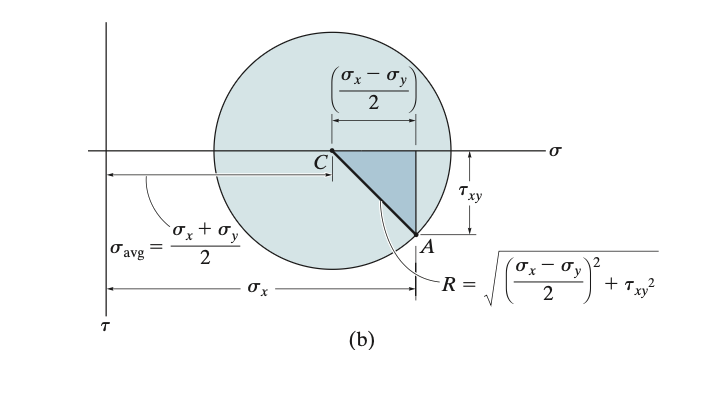
\includegraphics[width=0.8\linewidth]{./figures/f24_15.png}
  \caption{Mohr's circle.}
  \label{fig:f24_15}
\end{figure}

Each point on Mohr's circle represents the two stress components $\sigma_{x'}$ and $\tau_{x'y'}$ acting on the side of the element defined by the outward $x'$ axis, when this axis is in a specific direction $\theta$.

\subsection{Absolute Maximum Shear Stress}
The strength of a ductile material depends upon its ability to resist shear stress.
Therefore, it is important to find the absolute maximum shear stress in a material subject to a loading.

When $\sigma_1$ and $\sigma_2$ have the same sign the maximum absolute shear stress is:
\begin{equation*}
  \tau_{\text{abs max}} = \frac{\sigma_1}{2}
.\end{equation*}

When $\sigma_1$ and $\sigma_2$ have opposite signs the maximum shear stress is:
\begin{equation*}
  \tau_{\text{abs max}} = \frac{\sigma_1 - \sigma_2}{2}
.\end{equation*}


